\section*{Introduction}
In this chapter, we will examine in detail the key technologies that are used in our solution to provide advanced features and meet the specific needs of our project. The three main technologies we will cover are Delta Lake, Trino, and Microfrontends.

\section{Delta Lake}

Delta Lake is a data management technology that enables efficient and reliable storage, management, and analysis of massive volumes of data. It is built on a file-based Parquet architecture and offers advanced features such as ACID (Atomicity, Consistency, Isolation, Durability) transaction management and compatibility with popular analytics tools. Delta Lake also ensures data integrity, query consistency, and supports replication and recovery in case of failures.

The concept of a `lakehouse' is made possible by Delta Lake. It is a data architecture that combines the benefits of data warehouses and data lakes, providing a unique and consistent approach to data management. Data is stored in Parquet format in the data lake, enabling continuous and batch processing.
\begin{itemize}
\item \textbf{Enables Lakehouse architecture:} Delta Lake enables a continuous and streamlined data architecture that allows organizations to manage and process massive volumes of data in a continuous and batch manner without the hassle of separately managing and operating streaming, data warehouses, and data lakes.
\item \textbf{Enables intelligent data management for data lakes:} Delta Lake provides efficient and scalable metadata management, which provides insights into massive data volumes in data lakes. With this information, data governance and management tasks can be performed more effectively.
\item \textbf{Schema enforcement for improved data quality:} Since data lakes don't have a defined schema, it becomes easy for bad/incompatible data to enter the data systems. Data quality is improved through automatic schema validation, which validates DataFrame and table compatibility before writes.
\item \textbf{Enables ACID transactions:} Most organizational data architectures involve numerous ETL and ELT movements in and out of data storage, which opens it up to more complexity and failure points. Delta Lake ensures data durability and persistence during ETL and other data operations. Delta Lake captures all data changes during data operations in a transaction log, ensuring data integrity and reliability during data operations.
\end{itemize}

\cite{deltalake}

\section{Key Benefits and Features of Delta Lake}
\begin{flushleft}
With Delta Lake, data is stored in an optimized format, such as Parquet, in a data lake. This format enables efficient query processing regardless of the mode of data access, whether it is streaming or batch processing.
\end{flushleft}

\cite{databricksdelta}

\begin{figure}[H]
\centering
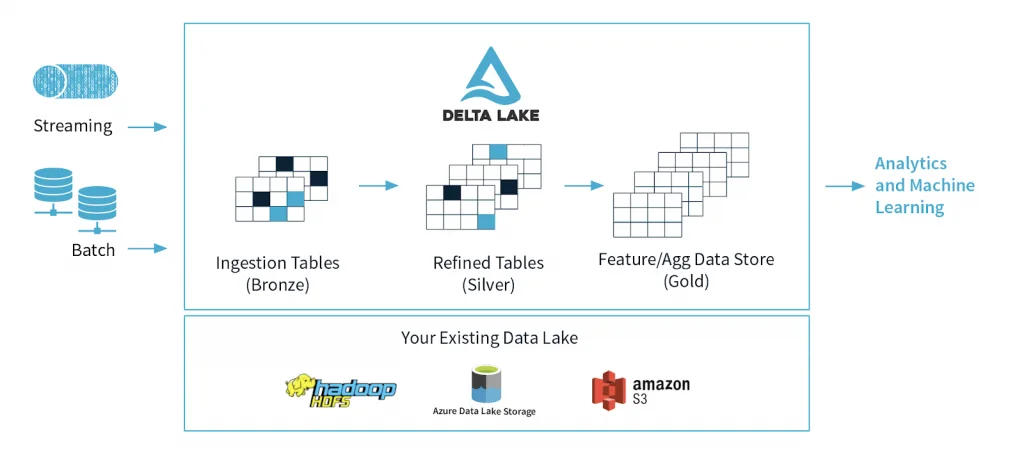
\includegraphics[width=\linewidth]{images/delta_lake_architecture.png}
\caption{Delta Lake multi-hop architecture}\label{fig:delta-lake-architecture}
\end{figure}

\begin{itemize}
\item[\textbullet] \textbf{Audit trails and history:} In Delta Lake, each write exists as a transaction and is sequentially recorded in a transaction log. Therefore, all modifications or validations made to the transaction log are recorded, leaving a complete trail to be used for historical audits, versioning, or time travel purposes. This Delta Lake feature ensures data integrity and reliability for enterprise data operations.
\item[\textbullet] \textbf{Time travel and data versioning:} Since each write creates a new version and stores the old version in the transaction log, users can view/restore old versions of data by providing the timestamp or version number of an existing table or directory to the Spark read API. Using the provided version number, Delta Lake then constructs a complete snapshot of the version with the information provided by the transaction log. Rollbacks and version management play a crucial role in machine learning experimentation, where data scientists iteratively modify hyperparameters to train models and can revert to previous changes if necessary.
\item[\textbullet] \textbf{Unifies batch and stream processing:} Each table in a Delta Lake is both a batch and stream sink. With Structured Streaming in Spark, organizations can efficiently stream and process data. Additionally, with efficient metadata management, scalability, and ACID quality for each transaction, near-real-time analytics becomes possible without using a more complicated two-tier data architecture.
\item[\textbullet] \textbf{Efficient and scalable metadata management:} Delta Lake stores metadata information in the transaction log and leverages the distributed processing power of Spark to quickly process, read, and manage large volumes of data metadata, thereby enhancing data governance.
\item[\textbullet] \textbf{ACID transactions:} Delta Lake ensures that users always see a consistent view of data in a table or directory. It achieves this by capturing every modification made in a transaction log and isolating it at the strongest isolation level, the serializable level. At the serializable level, every existing operation has and follows a serial sequence that, when executed one by one, provides the same result as stated in the table.
\item[\textbullet] \textbf{Data Manipulation Language (DML) operations:} Delta Lake supports DML operations such as updates, deletes, and merges, which play a role in complex data operations such as Change Data Capture (CDC), continuous upserts, and Slowly Changing Dimensions (SCD). Operations like CDC ensure data synchronization across all data systems and minimize time and resources spent on ELT operations. For example, using CDC, instead of ETL-ing all available data, only the recently updated data since the last operation undergoes transformation.
\item[\textbullet] \textbf{Schema enforcement:} Delta Lake performs automatic schema validation by checking a set of rules to determine the compatibility of a DataFrame write to a table. One such rule is the existence of all DataFrame columns in the target table. An occurrence of an extra or missing column in the DataFrame raises an error exception. Another rule is that the DataFrame and the target table must have the same column types, which, if not, triggers an exception. Delta Lake also uses Data Definition Language (DDL) to explicitly add new columns. This data lake feature helps avoid the ingestion of incorrect data, ensuring high data quality.
\item[\textbullet] \textbf{Compatibility with Spark API:} Delta Lake is built on Apache Spark and is fully compatible with the Spark API, enabling the creation of efficient and reliable large-scale data pipelines.
\item[\textbullet] \textbf{Flexibility and integration:} Delta Lake is an open-source storage layer and utilizes the Parquet format for storing data files, which promotes data sharing and facilitates integration with other technologies, fostering innovation.
\end{itemize}

\section{Trino}

Trino, formerly known as Presto, is a distributed, open-source SQL query engine. It is designed to execute interactive and analytical queries at a large scale on heterogeneous and distributed data. Trino offers great versatility by allowing access to various types of data sources, whether they are relational databases, file systems, real-time data sources, or cloud storage services. With its distributed design, Trino enables high performance and horizontal scalability, making it an essential tool for data analysis in our solution.

\cite{trino}

\begin{figure}[H]
\centering
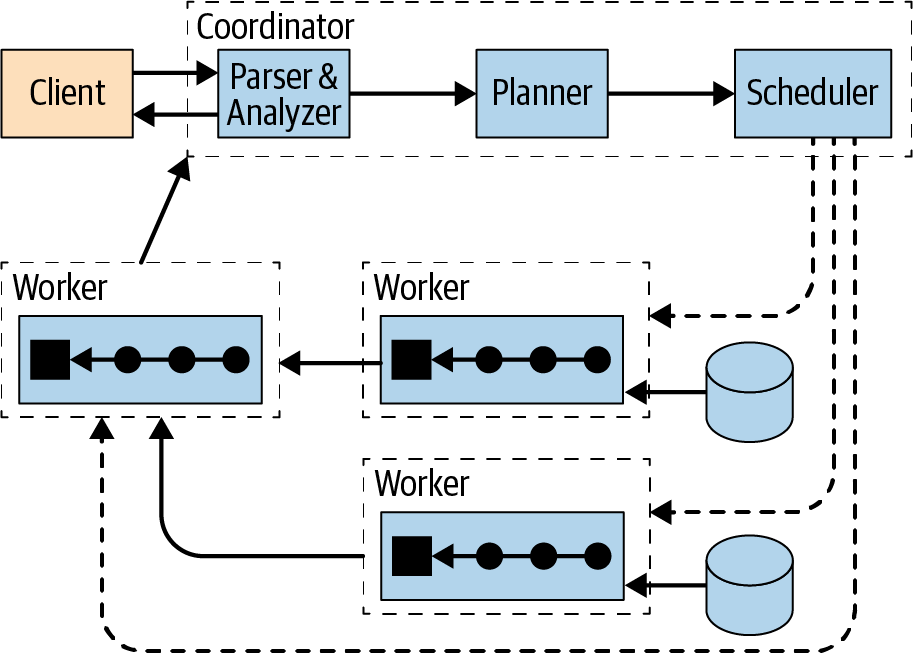
\includegraphics[width=0.8\linewidth]{images/trino_architecture.png}
\caption{Overview of Trino architecture with coordinator and workers}\label{fig:trino-architecture}
\end{figure}

\begin{enumerate}
\item A coordinator is a Trino server that handles incoming queries and manages workers to execute the queries.
\item A worker is a Trino server responsible for executing tasks and processing data.
\item The discovery service typically runs on the coordinator and allows workers to register to participate in the cluster.
\item All communications and data transfers between clients, the coordinator, and workers use REST-based interactions over HTTP/HTTPS.
\end{enumerate}

\section{Spring Boot}

Spring Boot is an open-source framework for Java application development. It provides a simplified and opinionated approach to creating standalone, production-ready Java applications without the need for complex configuration.

One of the main advantages of Spring Boot is its ability to reduce boilerplate configuration and simplify application development by providing smart default configuration definitions and automating many development tasks. It also embeds an application server, making it easy to deploy and run the application without requiring an external application server.

Spring Boot follows the annotation-driven programming paradigm, where annotations are used to configure and orchestrate different parts of the application. It offers a wide range of features, such as dependency injection, externalized configuration, error handling, security, data access, etc. These features are bundled into starters, which are pre-defined dependencies that facilitate adding specific functionality to the application.

With its simplified approach, Spring Boot allows developers to focus more on the business logic of their application rather than tedious configuration tasks. It also promotes good development practices, such as separation of concerns and modularity, making applications more maintainable and scalable.

\cite{springboot}

\section{Keycloak}

Keycloak is an open-source Identity and Access Management (IAM) solution developed by Red Hat. It provides comprehensive features for user management, authentication, authorization, and securing applications.

Keycloak helps centralize and simplify identity management within an IT infrastructure. It offers features such as user registration, multi-factor authentication, role and permission management, session management, and integration with common authentication and authorization protocols like OAuth 2.0 and OpenID Connect.

Keycloak provides functionality for managing roles, administrators, users, and passwords. Here's how Keycloak addresses these aspects:

\cite{keycloak}

\begin{enumerate}
\item Keycloak allows defining roles at the realm or application level. Roles can be created and assigned to users to define their permissions and access.
\item Keycloak administrators can create, manage, and assign roles to users through the administration interface or management API.
\item Roles can be used to control access to features, pages, and resources within the application.
\item Keycloak provides specific administration roles like "admin" or "superadmin" that allow users to perform administrative tasks such as managing clients, users, roles, etc.
\item Users can log in using their credentials (username and password) or other supported authentication methods like two-factor authentication, OAuth 2.0, etc.
\item Keycloak supports user-based authentication and provides a registration interface to allow users to create their accounts.
\item Keycloak also offers advanced authentication features such as two-factor authentication, social authentication (via identity providers like Google, Facebook, etc.), and certificate-based authentication.
\end{enumerate}

\begin{figure}[H]
\centering
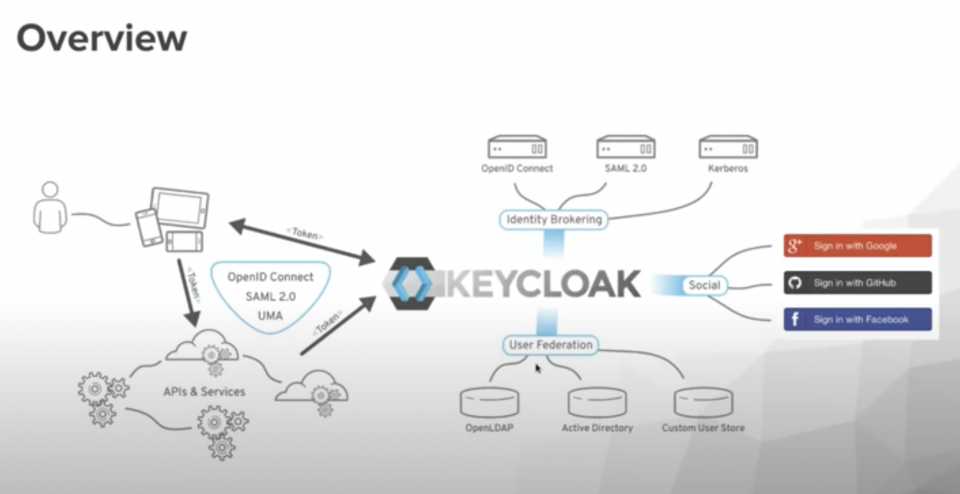
\includegraphics[width=\linewidth]{images/Keycloak-overview-screenshot.png}
\caption{Keycloak Overview}\label{fig:keycloak}
\end{figure}


\section{Kafka}

Kafka is a distributed and scalable data streaming platform designed to efficiently handle the transmission and processing of real-time data streams. It was developed by Apache Software Foundation.

Kafka is based on a distributed log architecture, where data is stored as streams of messages in "topics". Data producers send messages to specific "topics," while consumers subscribe to those "topics" to retrieve the messages. This allows for asynchronous communication and clear separation between data producers and consumers.

\cite{kafka}

The key features of Kafka include:

\begin{enumerate}
\item Scalability: Kafka is designed to handle large volumes of data and can be horizontally scaled to meet growing performance needs. It can handle high workloads and process thousands of messages per second.
\item Fault tolerance: Kafka ensures high availability and fault tolerance by replicating data across multiple nodes in the cluster. This ensures data reliability and availability even in case of node failures.
\item Data durability: Messages stored in Kafka are persistent and can be retained for a defined period. This allows for message replay and data recovery when needed, which is crucial for use cases requiring long-term data retention.
\item Stream processing: Kafka is designed for real-time stream processing. It enables applications to consume continuous data streams and process them in real-time, which is critical for use cases requiring real-time analysis, data pipelines, etc.
\item Integration with other tools: Kafka easily integrates with other tools and frameworks such as Spark, Hadoop, Flink, etc. This enables seamless integration with the Big Data ecosystem and facilitates data ingestion, processing, and streaming.
\end{enumerate}

\begin{figure}[H]
\centering
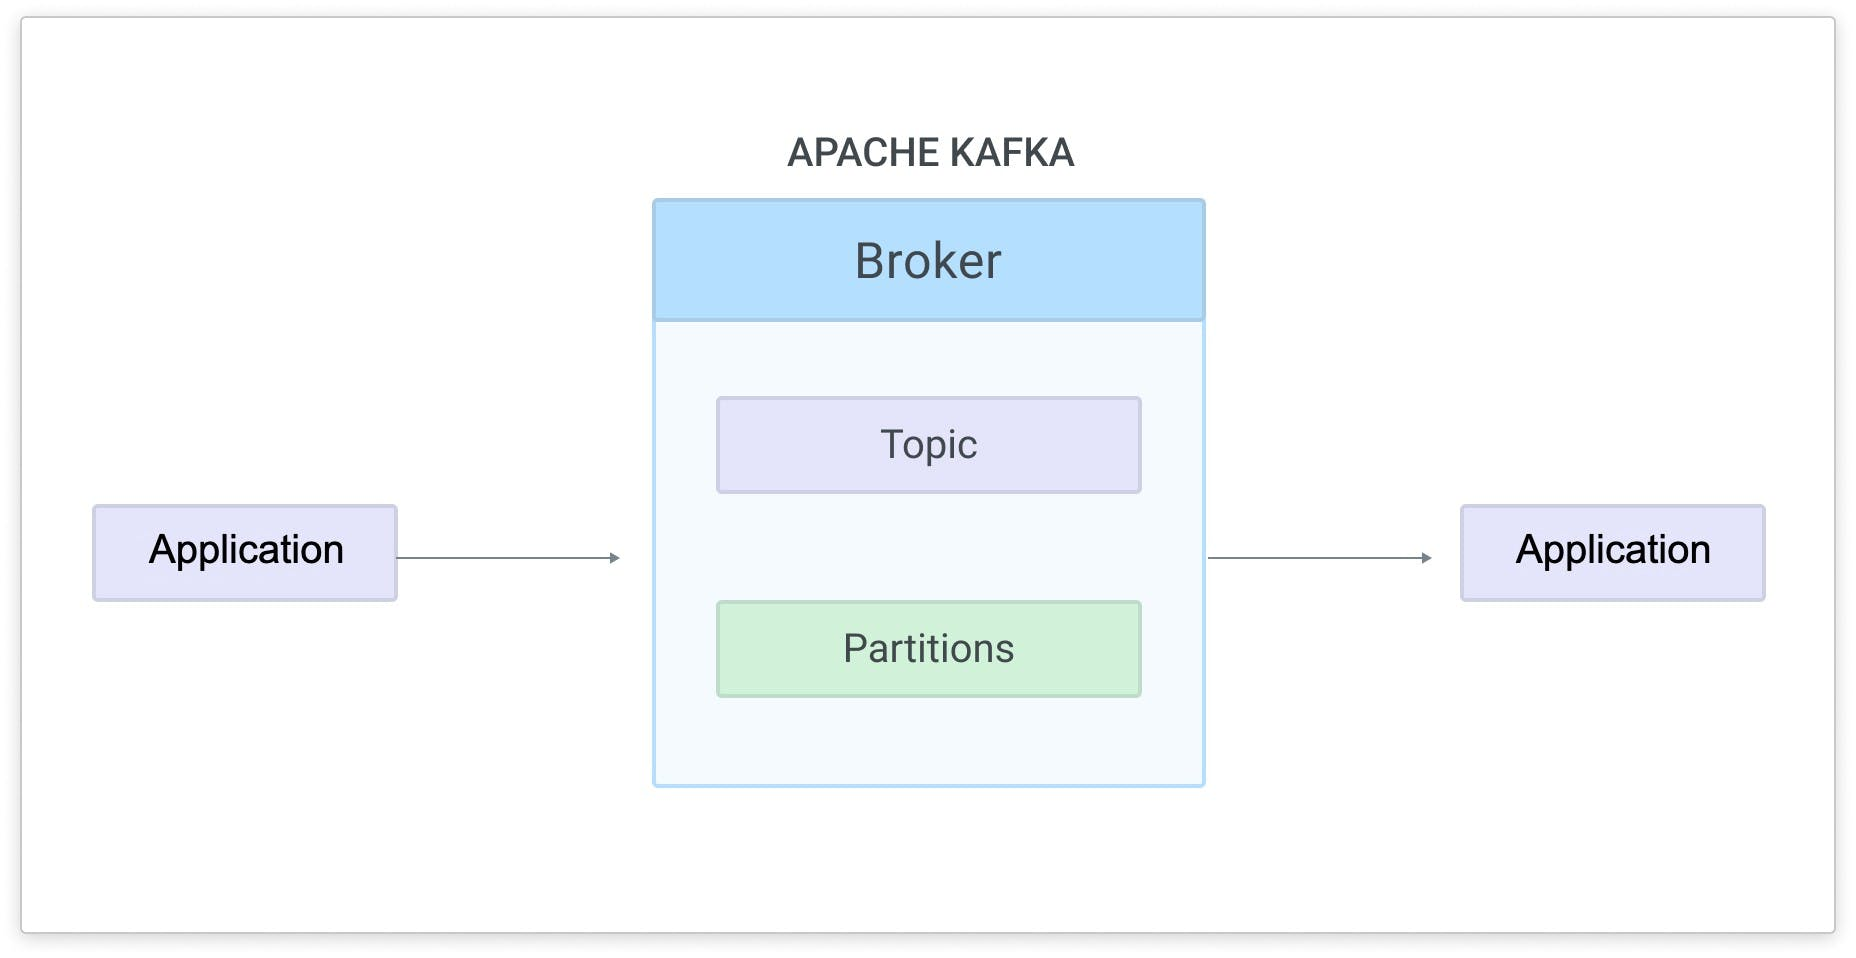
\includegraphics[width=\linewidth]{images/kafka.jpg}
\caption{Kafka Architecture}\label{fig:kafka}
\end{figure}

\section*{Conclusion}
these technologies, developers and data professionals can leverage their strengths to build powerful and scalable applications. Trino enables fast and flexible data querying, Spring Boot simplifies application development, Keycloak provides robust IAM capabilities, and Kafka enables real-time data streaming and processing.